\chapter{Experiments} % (fold)
\label{chap:experiments}
In this chapter the validation of the ping pong ball catchers ability to determine the point of impact on the base plate and being able to move to catch the ball after a ball bounce back.
\section{Catching the ball in time}
In order to validate that the calculations and movement of the servo is fast enough to catch a ping pong ball after a bounce back after a drop from $30\si{\centi\meter}$. The ping pong ball is dropped over the center of the plate, where the positioning system often calculates the impact point to be. The arm goes in and catches the ball in without troubles. 
Based on this result it is concluded that the timing constrains on calculating where the arm should move to and moving it there are satisfied.
\section{Positioning}
In order to test whether the positioning system calculates the correct position tests were conducted.
In each test a ball is dropped on to the same position on the base plate. The target is 30 degrees from the x-axis and a distance of the arms length from the origo. This target is marked with a red dot on figure \ref{fig:testRes30deg}. 
As can be seen in the figure the positions of the impact points are calculated to be at very different places at the different attempt of dropping the ball at almost the same point.
\begin{figure}[htb]
	\centering
	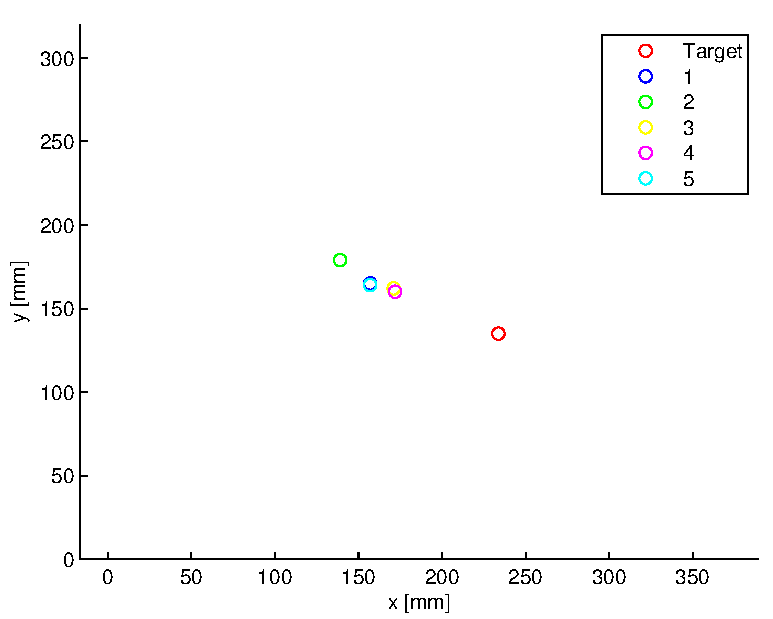
\includegraphics[width=.8\textwidth]{figures/testRes30deg.pdf}
	\caption{Estimated impact positions based as a result of dropping a ball on to the same target multiple times.}
	\label{fig:testRes30deg}
\end{figure}
The reason to this error is differences in the timings as can be seen in figure \ref{fig:clockCycles30deg}. In the figure the time difference between the four measurements on respectively sensor a, b, c and d. Which is indicated as blue, cyan and yellow. The measurements on d cannot be seen since they are zero for all the measurements. As can be seen the measurements are all over the place.

\begin{figure}[htb]
	\centering
	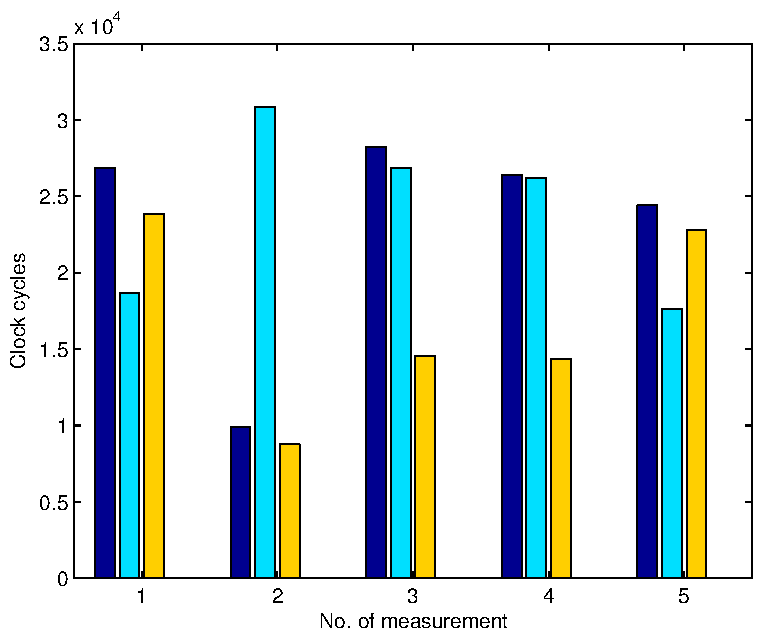
\includegraphics[width=.8\textwidth]{figures/clockCycles30deg.pdf}
	\caption{Estimated impact positions based as a result of dropping a ball on to the same target multiple times.}
	\label{fig:clockCycles30deg}
\end{figure}

\section{Unstable to small changes in time}
To validate the timings the timing results from the timing VHDL component are compared with time difference calculated based on sampling the same sensor output on an oscilloscope. The sensor output can be seen on figure \ref{fig:timingPlot}. 
\begin{figure}[htb]
	\centering
	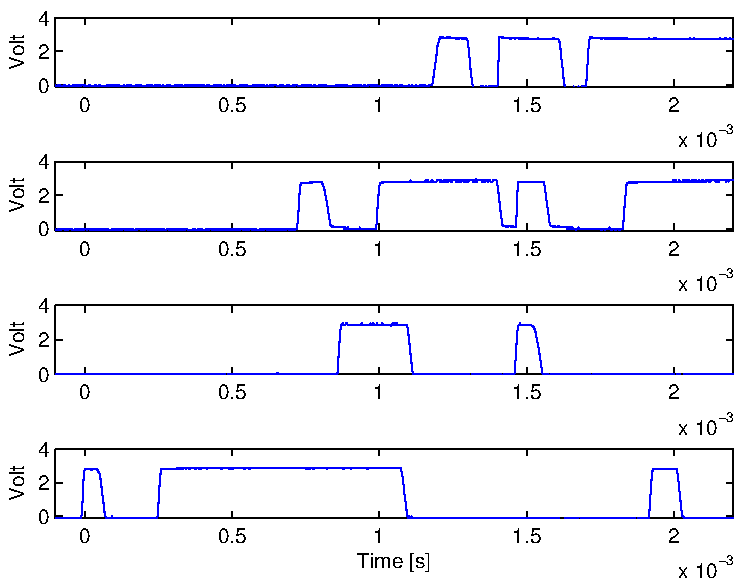
\includegraphics[width=.8\textwidth]{figures/timingPlot.pdf}
	\caption{Estimated impact positions based as a result of dropping a ball on to the same target multiple times.}
	\label{fig:timingPlot}
\end{figure}
Timings to compare with are extracted by running through the sequence from the beginning until a value larger than the 2.4V are reach. The time at these points are stored for each sensor. The compare time values in table \ref{tbl:compareCycles} can be calculated by multiplying the time difference between each of the stored times and the smallest of them with the clock frequency the timing component counts with(50Mhz). 
%
\begin{table}[h]
	\begin{tabular}{|l|l|l|l|l|}
		\hline		
		 & ta & tb & tc & td \\
		 \hline		
		Difference in cycles from timing module & 36655 & 59827 & 43481 & 0 \\	
		 \hline
		Difference in cycles from oscilloscope & 36600 &  60000 &  43400 & 0 \\		
		\hline				
	\end{tabular}
	\caption{Comparison of clock cycles from timing module and calculated from oscilloscope data.}
	\label{tbl:compareCycles}
\end{table}
%
As can be seen from table \ref{tbl:compareCycles} the compare values are roughly the same. Hence it is concluded that the timing is correct, so the fault must be before the FPGA in the system.
% chapter experiments (end)